\subsection{Perfect Placement for Your AC Surge Protector!}

\begin{tcolorbox}[colback=gray!10, colframe=black, title=E4E13]

Where should a station AC surge protector be installed?
\begin{enumerate}[label=\Alph*.]
    \item At the AC service panel
    \item At an AC outlet
    \item \textbf{On the single point ground panel}
    \item On a ground rod outside the station
\end{enumerate} \end{tcolorbox}

\subsubsection{Related Concepts}

To correctly answer this question, it’s crucial to understand the purpose of an AC surge protector and the principles of grounding in electrical systems. An AC surge protector is designed to absorb or divert excess voltage surges, often caused by lightning strikes or power fluctuations, thereby protecting sensitive electronic equipment connected to the AC circuit. 

The term “single point ground” refers to a grounding methodology where all equipment is connected to a single grounding point, minimizing ground loops and differences in potential that can cause interference and equipment failure.

\subsubsection{Grounding Principles}

Grounding is an essential practice in electrical installations that ensures safety and proper functioning of electrical equipment. Here are key points to consider:

1. \textbf{Purpose of Grounding}: Grounding provides a path of least resistance for electrical faults, thus preventing electrical shock hazards and damage to equipment.
2. \textbf{Single Point Grounding}: This technique ensures that all equipment is referenced to one single ground point, avoiding issues such as ground loops which can introduce noise and interference in signal integrity.

\subsubsection{Installation Recommendations}

When installing an AC surge protector, the best practice is to install it on the single point ground panel for several reasons:

- It allows for effective dissipation of surges to the ground.
- It minimizes the potential difference between various pieces of equipment, enhancing operational stability.
- It serves as a centralized point for managing AC protection.

\subsubsection{Calculation Example}

While a calculation may not be strictly required in this scenario, understanding the voltage levels and surge ratings for different devices connected through the surge protector is important. If necessary, you can estimate the surge energy absorption requirement using the following relationship:

\[
E = \frac{V^2}{R}
\]

Where:
- \(E\) is the energy in joules
- \(V\) is the voltage (in volts)
- \(R\) is the resistance (in ohms)

However, in practice, manufacturers often specify maximum voltage ratings and energy absorption capacity for surge protectors, which can guide their selection based on the expected electrical environment.

\subsubsection{Diagram}

\begin{center}
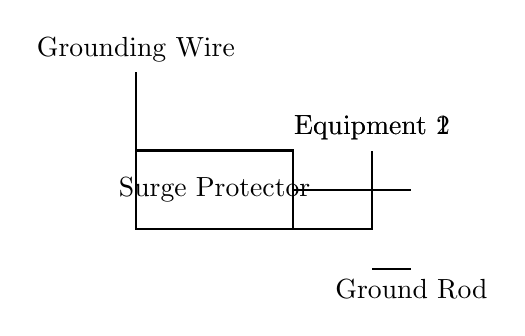
\begin{tikzpicture}
    % Grounding Diagram
    \draw[thick] (0,0) rectangle (2,1) node[pos=.5] {Surge Protector};
    \draw[thick] (0,1) -- (0,2) node[above] {Grounding Wire};
    \draw[thick] (2,0.5) -- (3,0.5) -- (3,1) node[above] {Equipment 1};
    \draw[thick] (2,0) -- (3,0) -- (3,1) node[above] {Equipment 2};
    \draw[thick] (3,0.5) -- (3.5,0.5);
    \draw[thick] (3,-0.5) -- (3.5,-0.5) node[below] {Ground Rod};
\end{tikzpicture}
\end{center}

This diagram illustrates the placement of an AC surge protector connected to various pieces of equipment, with a grounding line connecting to the ground rod, ensuring effective surge protection.
